\subsection{Simplified motor model}
The motor that requires controlling is a "Motenergy ME1117 PMAC Motor", that is driving force of the go kart supplied by SDU. The parameters of the motor is in the table below.

\begin{table} [H]
\centering
\begin{tabular}{|c|c|} \cline{1-2}
\textbf{Parameters} & \textbf{Number} \\ \cline{1-2}
\textbf{Pole pair} & $4\ pairs\ (8\ poles)$ \\ \cline{1-2}
\textbf{Phase to Phase R} & $0.013\ohm$ \\ \cline{1-2}
\textbf{Maximum rotational speed} & $5000$ \textit{RPM} \\ \cline{1-2}
\textbf{Voltage rating} & $0-76$ \textit{Volts} \\ \cline{1-2}
\textbf{Torque constant} & $0.13$ \textit{Nm/A} \\ \cline{1-2}
\textbf{Inductance Phase to Phase} & $0.1$ \textit{mH} \\ \cline{1-2}
\textbf{Armature Inertia} & $52\ kg/cm^2$ \\ \cline{1-2}
\textbf{Continuous current} & $100\ A$ \\ \cline{1-2}
\textbf{Peak Current for 1 min} & $300\ A$ \\ \cline{1-2}  
\end{tabular} \\
\caption{Motor parameters as seen in \cite{Motor_Parameters}}
\label{Motor_parameters_list}
\end{table}

\begin{figure}
    \centering
    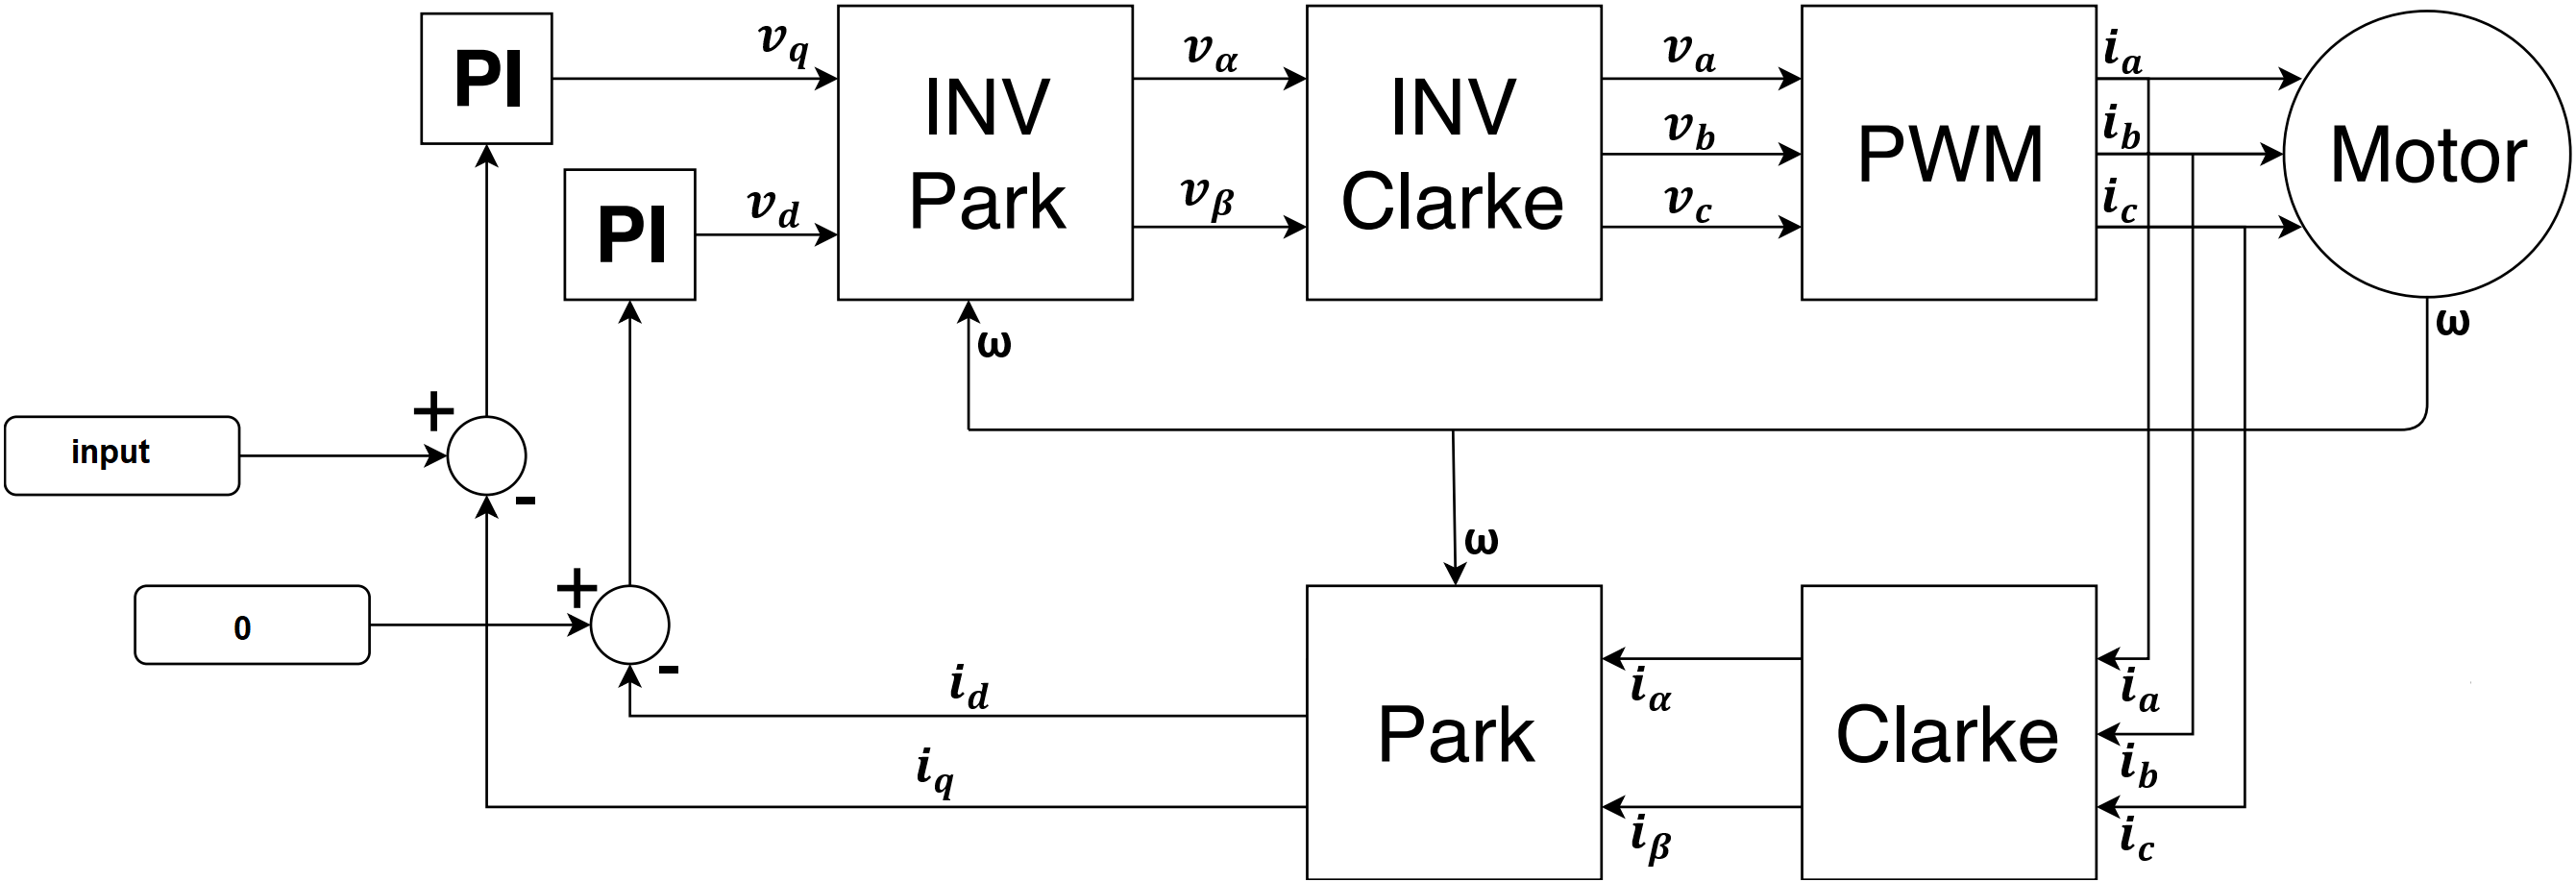
\includegraphics[scale=0.25]{pictures/control/udklip.PNG}
    \caption{Motor model used for the control in an overview}
    \label{fig:my_label}
\end{figure}{}